\documentclass{a0poster}
\usepackage[dvipsnames,svgnames]{xcolor}
\usepackage{tikzposter} % here most of the things are defined
% change parameters only after this line You can also start a new column with an arbitrary 
% x-coordinate by specifying explicitly the coordinate of the new block node as follows:
\usepackage[czech]{babel}
\usepackage[utf8]{inputenc}
\usepackage{wrapfig}
\usepackage{url}

\usepackage[margin=\margin cm, paperwidth=84.1cm, paperheight=118.9cm]{geometry}

% \setbackgrounddarkcolor{ForestGreen!70!black}
% \setbackgroundlightcolor{YellowGreen!90!}

% \setfirstcolor{YellowGreen!80!}
% \setsecondcolor{gray!80!}
% \setthirdcolor{red!80!black}

\title{GRASS image processing environment\\ Gearing towards GRASS 7}
\author{Yann Chemin\\
International Water Management Institute}

\usetemplate{1}
\setinstituteshift{1}

\setblocktitleheight{2}
\setblockspacing{1}

\begin{document}
\ClearShipoutPicture
\AddToShipoutPicture{\BackgroundPicture}
\noindent
\tikzstyle{every picture}+=[remember picture]
\begin{tikzpicture}
\initializesizeandshifts
\titleblock{73.8}{1}
% \setblocktitleheight{1}

\addlogo[north west]{(2,-1)}{9cm}{./images/Grass_GIS.pdf}
\addlogo[north east]{(-2,-2.5)}{11cm}{./images/IWMI_logo.pdf}

\blocknode{Abstract}{
\small GRASS 7 started its development by the branching out of GRASS 6.x from the main trunk of code (rev 31142).
This was done on 27th of April 2008, and a large amount of changes took place since that date, more 
are still underway.
\begin{itemize}
 \item Display library in GRASS 7 (planning \& ongoing)
 \item Raster library in GRASS 7 (planning \& ongoing)
 \item Vector library in GRASS 7 (planning \& ongoing)
 \item G3d (volume) library and modules in GRASS 7 (finished)
 \item Temporal extension for GRASS 7 (finished) 
\end{itemize}

GRASS GIS capacity in remote sensing has also been under great changes and additions for version 7.
}

\blocknode{Linear features extraction}{
\small
An edge is considered as a change in image digital values.
Edge detection \& extraction in i.canny is done by a Canny edge detector [1]. 
The Canny edge detector encompasses Gaussian smoothing, 
gradient computation \& non-maximum suppression. \newline
This creates thin edges and thresholding with hysteresis which
preserves only important edges. Thus, no pre- or post-processing is required.
The produced binary image shows boundaries of areas in the input image
which is usually a gray scale image e.g., intensity channel or the
result of PCA.\newline
The i.edge module is suitable as a first step in building or road detection.
The level of details of the output image is easily customizable.
\begin{center}
 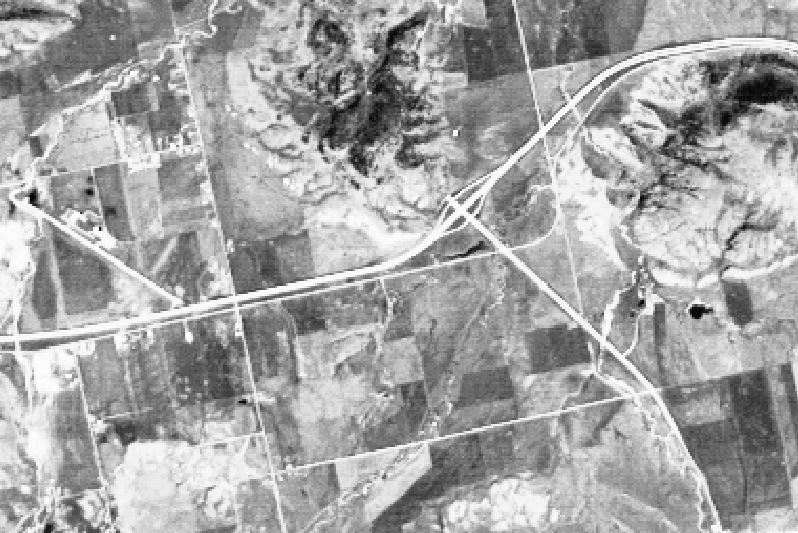
\includegraphics[width=0.48\textwidth]{./images/imagery_spot_original}
 \hspace{10mm}
 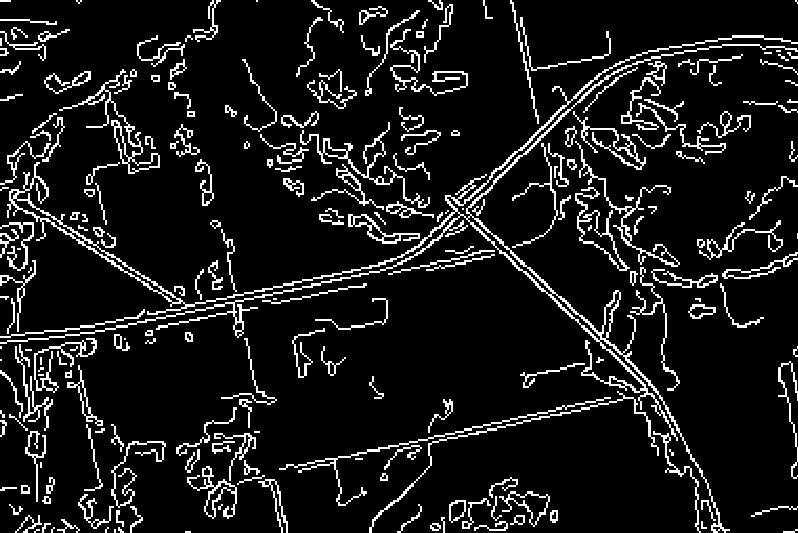
\includegraphics[width=0.48\textwidth]{./images/imagery_spot_edge_1}
 \newline
 Figure 1: Canny edge detector on a road network [1]
\end{center}
}

\blocknode{Object recognition}{
\small The module i.segment is a region growing image segmentation algorithm [2].
It produces a raster map with segments (objects), and optionally other maps with segments statistics 
(mean/variance/range/etc.). 
\begin{center}
 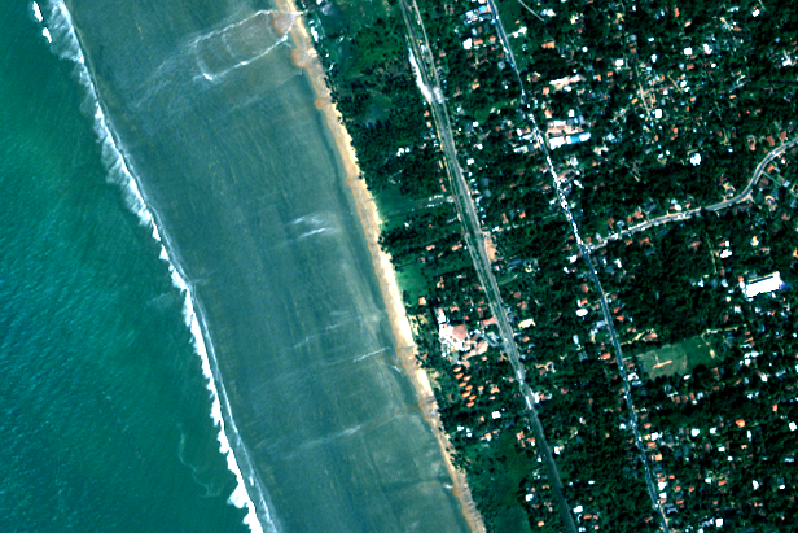
\includegraphics[width=0.48\textwidth]{./images/sltsu.png}
 \hspace{10mm}
 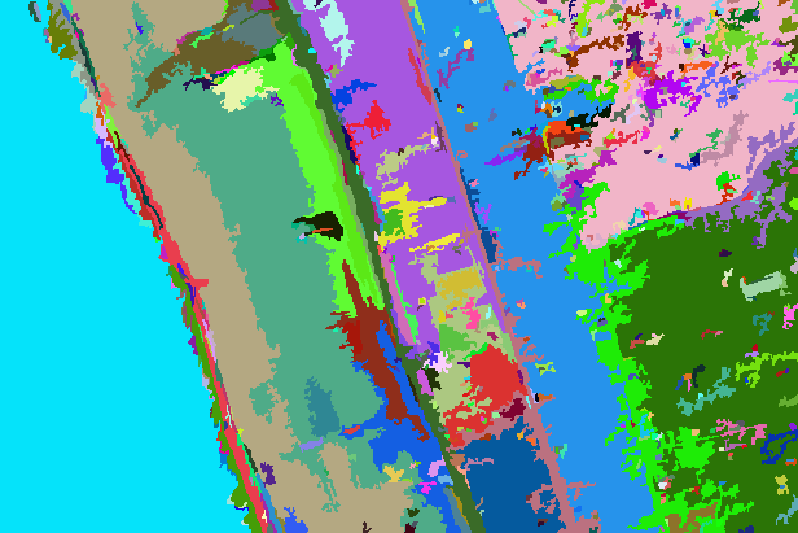
\includegraphics[width=0.48\textwidth]{./images/sltsu_seg.png}
 \newline
 Figure 2: Image segmentation (2.4x2.4m) of the 2004 tsunami wave, West Coast Sri Lanka
\end{center}
}

\blocknode{Satellite imagery products}{
\innerblockplain[colortwo!80!]{
\small
\begin{itemize}
 \item {\bf i.vi} 15 vegetation indices available
 \item {\bf i.albedo} Broadband Albedo (snow \~= 0.6-0.8, water=0.05)
 \item {\bf i.emissivity} Emissivity approximation from vegetation index
 \item {\bf i.biomass} biomass growth for crop yield
\end{itemize}

{\bf Reference/Potential ET: i.evapo.* modules}

\begin{itemize}
 \item {\bf i.evapo.mh} ETo Hargreaves, modified-Hargreaves \& Hargreaves-Samani 
 \item {\bf i.evapo.pm} ETo Penman-Monteith
 \item {\bf i.evapo.pt} ETpot Priestley-Taylor
\end{itemize}

{\bf Actual ET: i.eb.* modules using thermodynamic heat flux modeling}

% \begin{equation}\label{eq1}
% \Lambda = \frac {Rn - G - H} {Rn - G}
% \end{equation}
% 
% \begin{equation}\label{eq2}
% ET_a = \Lambda \, ET_{potential}
% \end{equation}

\begin{center}
 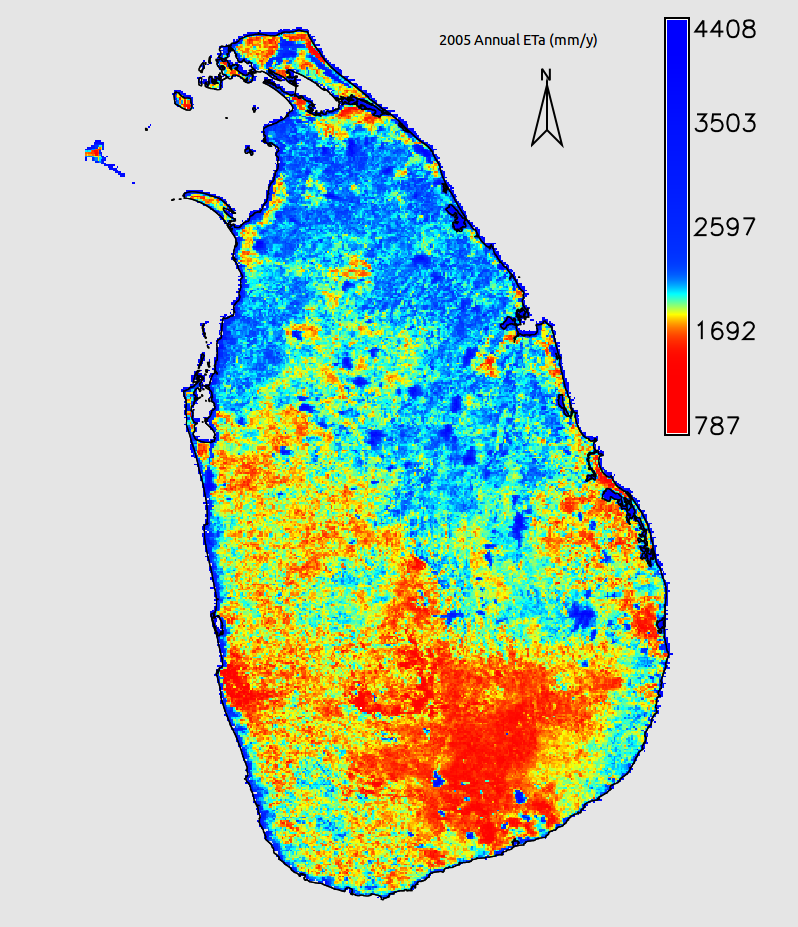
\includegraphics[width=0.38\textwidth]{./images/slet2005}
 \hspace{20mm}
 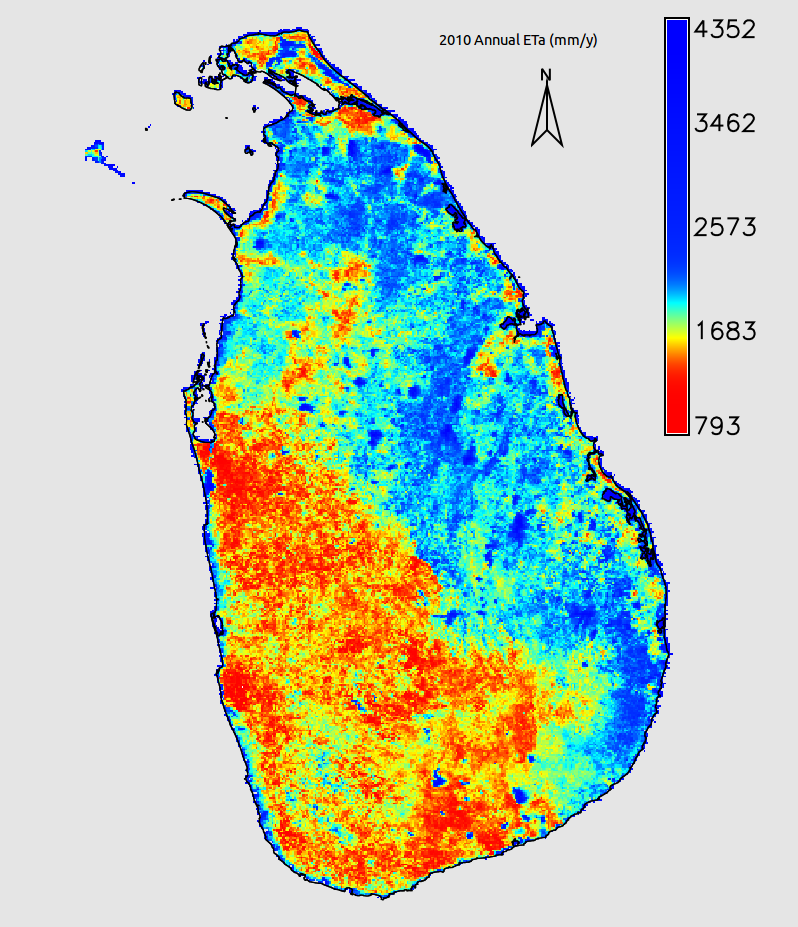
\includegraphics[width=0.38\textwidth]{./images/slet2010}
 \newline
 Figure 3: Actual evapotranspiration (i.eb.*) for water monitoring and management [3]
\end{center}
}
\vspace*{-25pt}
}


\startsecondcolumn


\blocknode{Interactive supervised classification}{
\innerblockplain[colortwo!80!]{
\small 
This interactive tool [4], aims at greatly simplifying quantitative surpervised class training areas creation.
It calculates the spectral signatures based on the cells within the specified areas. 
The resulting signature file can be used by a maximum likelihood classification module (i.maxlik). 
During the process the user is shown a histogram of the area cell values for each image band, 
and coincident plot which shows the separability of classes.\newline
Another way the user can inspect the suitability of the created training areas 
is by displaying the cells of the image bands which fall within a user-specified 
number of standard deviations from the means in the spectral signature. This
helps to estimate how much of the image is likely to be classified as a particular class.\newline
\begin{center}
 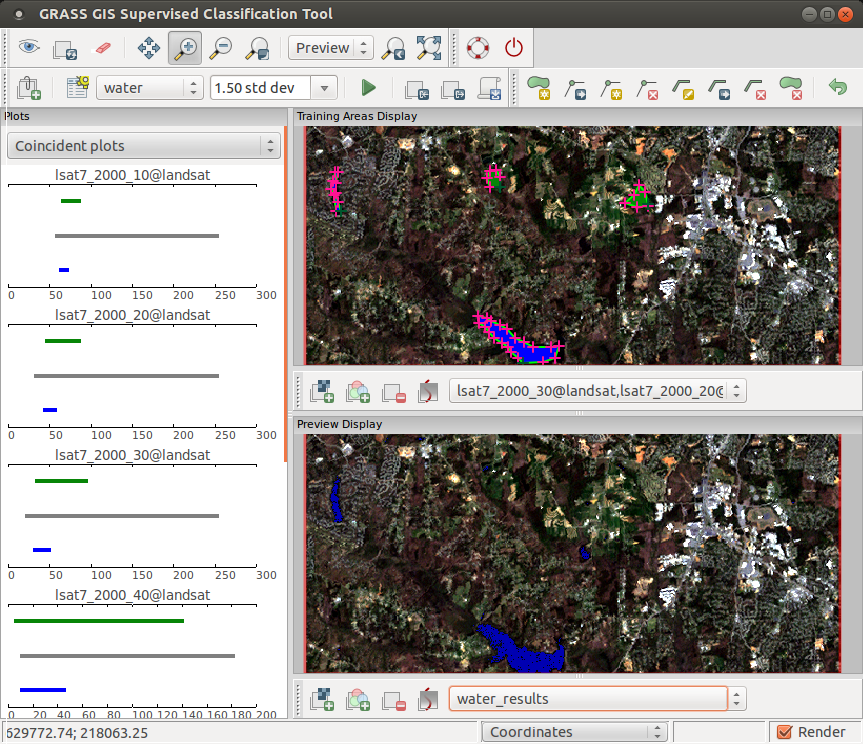
\includegraphics[width=0.47\textwidth]{./images/wxiclass1.png}
 \hspace{10mm}
 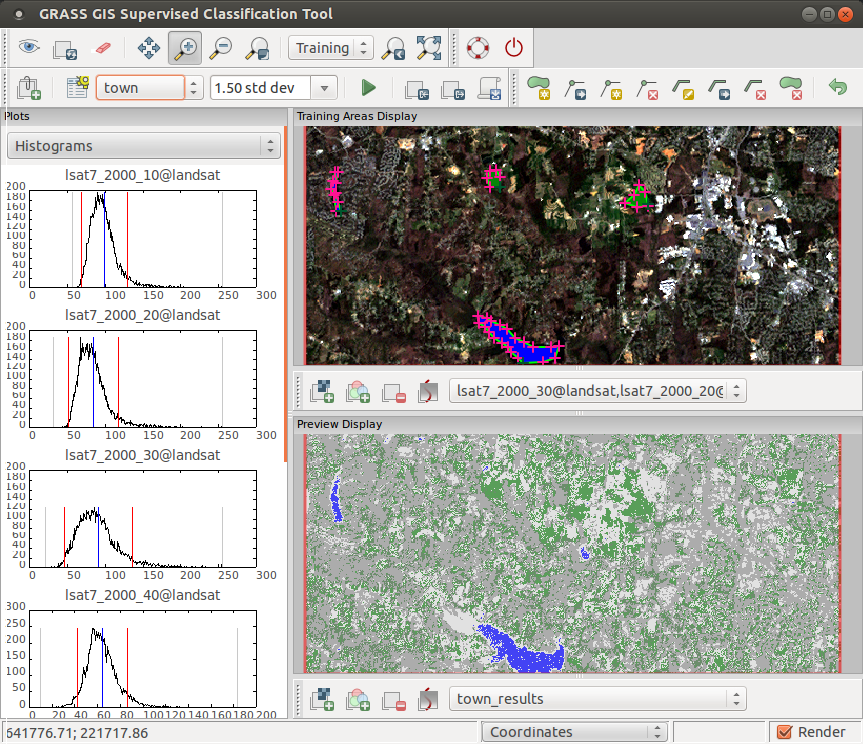
\includegraphics[width=0.47\textwidth]{./images/wxiclass2.png}
 \newline
 Figure 4: Interactive image classification with coincidence plots (left side) \& histograms (right side)
\end{center}
}
\hspace*{-25pt}
}

\blocknode{Lidar}{
\medskip
\innerblockplain[colortwo!80!]{
\small The Lidar library ({\url {www.liblas.org}}) included in GRASS GIS permits the import of Lidar (.las)
data in raster (r.in.lidar using statistics of choice) or in vector format (v.in.lidar). 
Author Markus Metz tested r.in.lidar with a 705Gb .las file. \newline
On-farm water storage study with lidar data in NSW (Australia) permitted to develop the 
first full remote sensing monitoring methodology of water availability by a combination of 
lidar-based bathymetric survey and multi-source remote sensing water area regular survey [5].\newline
\begin{center}
 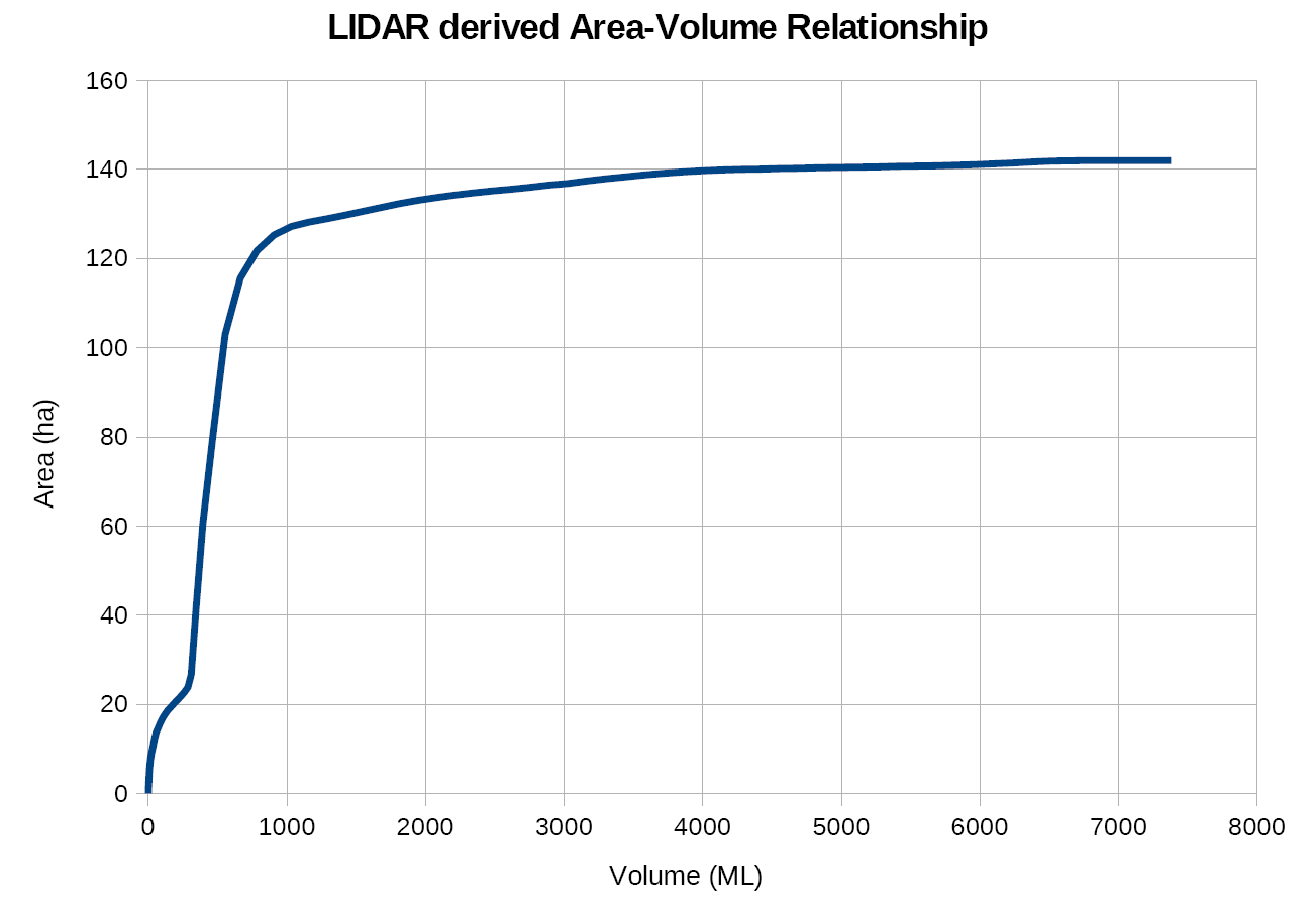
\includegraphics[width=0.4\textwidth]{./images/ofs1}
 \hspace{10mm}
 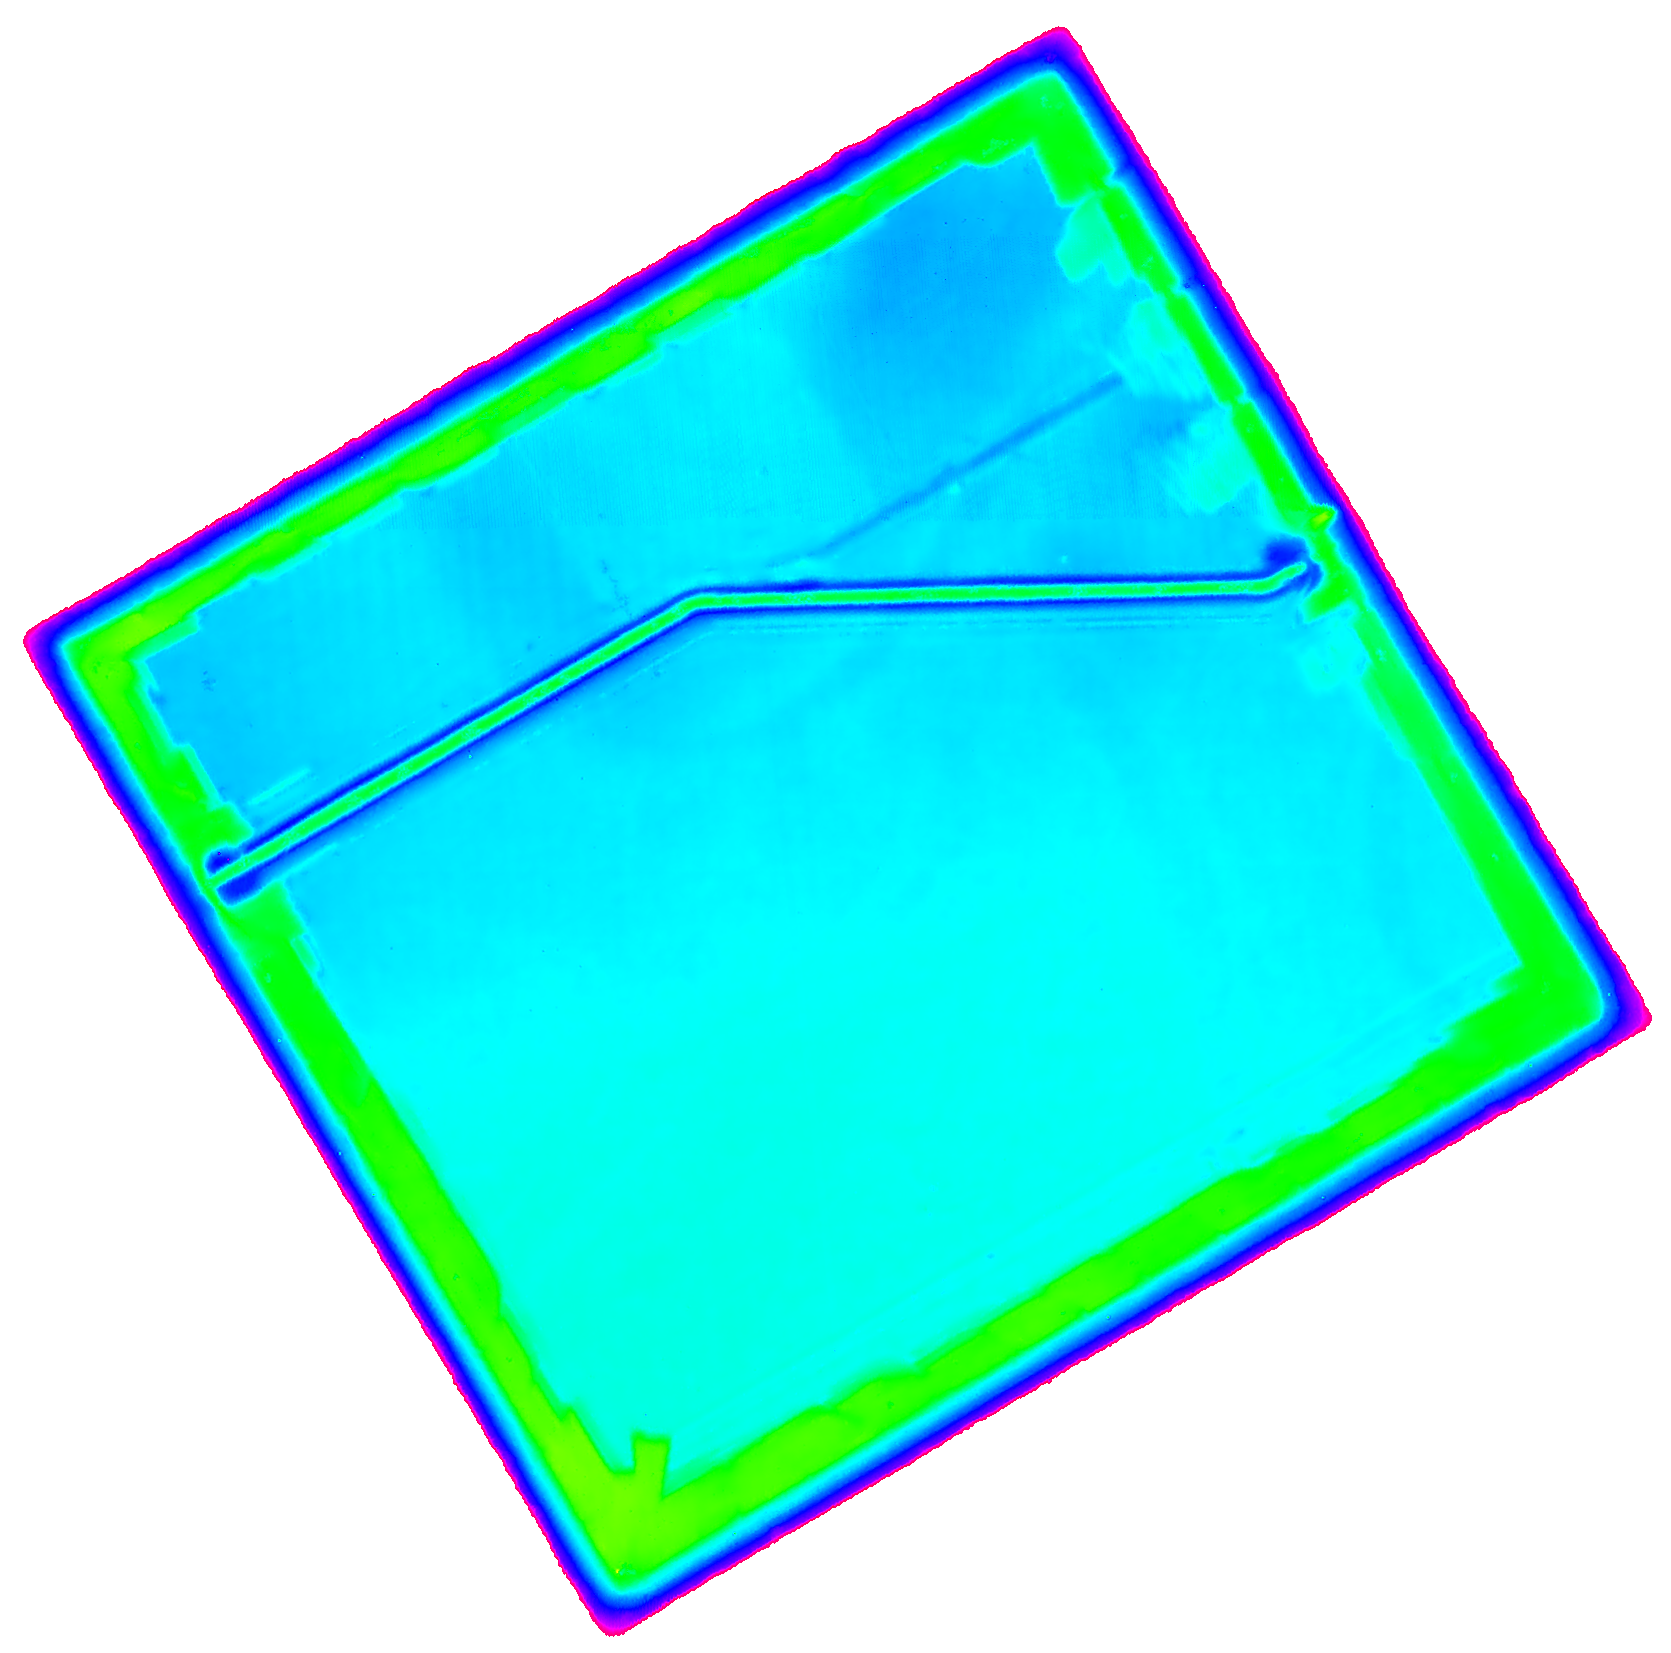
\includegraphics[width=0.275\textwidth]{./images/ofs2}
 \newline
 Figure 5: On-Farm-Water-Storage Lidar survey and Depth-Volume-Area surveying [5]
\end{center}
}
\vspace*{-25pt}
}
\blocknode{Other Improvements \& Additions}{
\medskip
\innerblockplain[colortwo!80!]{
\small 

{\bf Remanufacturing, performance improvement}

\begin{itemize}
 \item {\bf i.ortho.rectify} new rewritten \& optimized version of i.ortho.photo
 \item {\bf i.atcorr} atmospheric correction, more satellite sensors configured, faster
 \item {\bf i.pca} backward modeling implemented 
\end{itemize}
\vspace{15pt}
{\bf Preparing Landsat, Aster and MODIS datasets}

\begin{itemize}
 \item {\bf i.landsat.toar} TOA reflectance correction for Landsat satellite series
 \item {\bf i.aster.toar} TOA reflectance correction for Terra-ASTER
 \item {\bf i.modis.qc} Quality flag interpretation for Terra/Aqua MODIS
\end{itemize}
\vspace{15pt}
{\bf Geographical and astronomic functions}

\begin{itemize}
 \item {\bf i.latlong} maps latitude or longitude (dd.ddd)
 \item {\bf i.sunhours} maps potential hours of sunshine in a day at a given location (hh.hhh)
\end{itemize}
\vspace{15pt}
{\bf Temporal cleaning and smoothing}

A dedicated time-series environment (modules starting with t.*) is being developed for GRASS 7, 
the following functions initially developed for NDVI temporal interpolation and maximization might 
find their way in the t.* modules.
\begin{itemize}
 \item {\bf r.hants} Fourier temporal smoothing
 \item {\bf i.lmf} Local maximum fitting of temporal data
\end{itemize}
}
\vspace*{-25pt}
}

% \initializesizeandshifts
\getcurrentrow{box}
\coordinate (funkcionalita) at (box.south west);
\coordinate (funkcionalitaeast) at (box.east);
\coordinate (screenshot) at (box.north west);
% \getcurrentrow{box}
\blocknodew[($(funkcionalita)+(25,-1)$)]{25}{References}{
\scriptsize
\begin{center}
\begin{tabular}{rp{0.8\textwidth}}
[1] & Petráš, 2012. M.Sc. Thesis, OSGeoREL, FCE CTU, Prague.\\{}
[2] & Momsen \& Metz, 2012. i.segment module. Geographic Resources
Analysis Support System (GRASS GIS) Software, Version 7.\\{}
[3] & Chemin, 2012. Chapter 19, DOI: 10.5772/23571 ({\url {http://bit.ly/16qJOep}})\\{}
[4] & Kratochvílová \& Petráš, 2013. OSGeoREL, FCE CTU, Prague.\\{}
[5] & Chemin \& Rabbani, 2011. International Journal of Geoinformatics,  7(3):1-6pp.
\end{tabular}
\end{center}
\smallskip
\hrulefill
\vspace{-5pt}

\begin{center}
\begin{tabular}{cp{0.9\textwidth}}
\begin{minipage}{0.15\textwidth}

\includegraphics[width=0.7in]{./images/iwmi_qr.pdf}
\end{minipage}

\begin{minipage}{0.3\textwidth}
\small {\url{www.iwmi.org}}
\end{minipage}

\begin{minipage}{0.15\textwidth}

\includegraphics[width=0.7in]{./images/grass_qr.pdf}
\end{minipage}

\begin{minipage}{0.3\textwidth}
\small {\url{grass.osgeo.org}}
\end{minipage}
\end{tabular}
\end{center}

\hrulefill
\vspace{14pt}

\newcommand{\logowidth}{0.65em}
\newcommand{\logospace}{\hspace{0.1em}}
\noindent

\includegraphics[width=\logowidth]{./images/public_domain_logo.png}
\logospace Public Domain 2013 GRASS Development Team
}

\end{tikzpicture}

\end{document}
